\documentclass{standalone}
\usepackage{graphicx}	
\usepackage{amssymb, amsmath, amsthm}
\usepackage{color}

\usepackage{tikz}
\usetikzlibrary{intersections, backgrounds}

\definecolor{light}{RGB}{220, 188, 188}
\definecolor{mid}{RGB}{185, 124, 124}
\definecolor{dark}{RGB}{143, 39, 39}
\definecolor{highlight}{RGB}{180, 31, 180}
\definecolor{gray10}{gray}{0.1}
\definecolor{gray20}{gray}{0.2}
\definecolor{gray30}{gray}{0.3}
\definecolor{gray40}{gray}{0.4}
\definecolor{gray60}{gray}{0.6}
\definecolor{gray70}{gray}{0.7}
\definecolor{gray80}{gray}{0.8}
\definecolor{gray90}{gray}{0.9}
\definecolor{gray60}{gray}{0.95}

\begin{document}

\begin{tikzpicture}[scale=0.4, thick]

\begin{scope}[shift={(0, 0)}]
  \draw[white] (-8, -7) rectangle (8, 8);
    
  \begin{scope}
    \clip (-7, -7) rectangle (7, 6);
        \node at (0, 0) {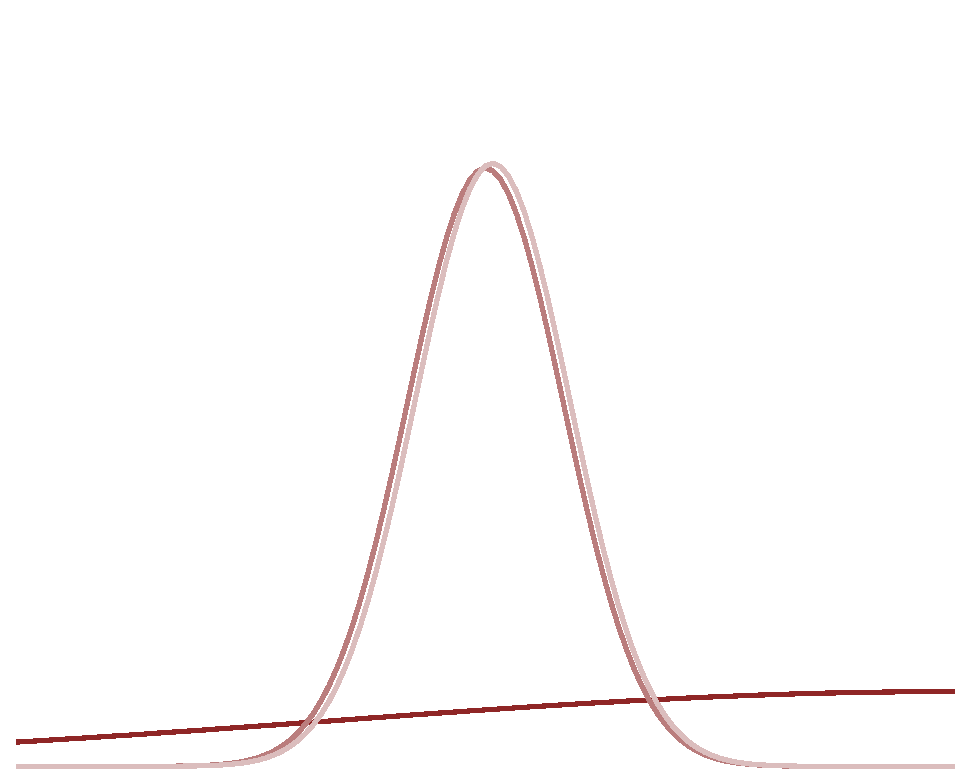
\includegraphics[height=4cm]{contraction_soft_zoom.eps}};
  \end{scope}
  
  \node[dark, align=center] at (4.5, -2.5) { Prior Density\\Function };
  \node[mid, align=center] at (-3, 1.5) { Likelihood\\Function};
  \node[light, align=center] at (4.25, 1.5) { Posterior Density\\Function };
  
  \node[align=center] at (0, 6) { Contraction with\\Soft Containment };
  
  \draw [<->, >=stealth, line width=1] (-7 - 0.025, -5) -- +(14, 0);
  \node[] at (0, -6) { $\theta$ };
\end{scope}

\begin{scope}[shift={(18, 0)}]
  \draw[white] (-8, -7) rectangle (8, 8);
    
  \begin{scope}
    \clip (-7, -7) rectangle (7, 6);
        \node at (0, 0) {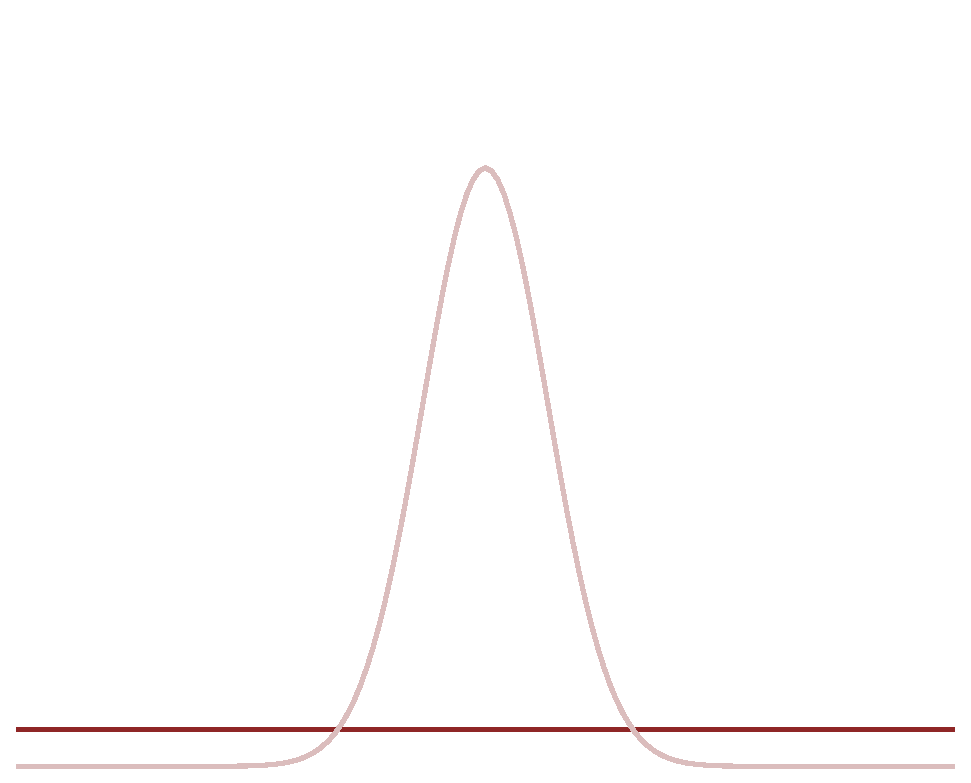
\includegraphics[height=4cm]{contraction_hard_zoom.eps}};
  \end{scope}
  
  \node[dark, align=center] at (4.25, -3) { Prior Density\\Function };
  \node[mid, align=center] at (-3, 1.5) { Likelihood\\Function};
  \node[light, align=center] at (4, 1.5) { Posterior Density\\Function };
  
  \node[align=center] at (0, 6) { Contraction with\\Hard Containment};
  
  \draw [<->, >=stealth, line width=1] (-7 - 0.025, -5) -- +(14, 0);
  \node[] at (0, -6) { $\theta$ };
\end{scope}

\end{tikzpicture}

\end{document}  